\documentclass[a4paper, 12pt]{article}
\usepackage[brazilian]{babel}
\usepackage{amsmath}
\usepackage{transparent}
\usepackage{graphicx} \graphicspath{{./images}}
\usepackage[colorlinks=true, linkcolor=blue]{hyperref}

\usepackage{csquotes}
\usepackage{biblatex}
\addbibresource{ref.bib}

\usepackage{tocloft}
\renewcommand{\cftdot}{\ensuremath{.}}
\renewcommand{\cftsecleader}{\cftdotfill{\cftdotsep}}

\title{Relatório de Projeto Final - Processador}
\author{Fernando Henrique Ratusznei Caetano}
\date{ }

\begin{document}
\maketitle
\tableofcontents

\newpage
\section{Introdução}

\par
Esse documento apresenta o projeto final realizado para a disciplina
EEB31, Circuitos Digitais, ministrada em conjunto pelos professores
Fabio Kurt Schneider e Bertoldo Schneider Junior.

\par
O projeto consiste de um sistema processador simplificado de 8 bits
e foi desenvolvido para ser executado em uma placa \textit{Terasic DE10-Lite}
utilizando o software \textit{Quartus Prime} versão 18.

\par
Esse projeto foi feito com base no livro "Digital Design and Computer Architecture RISC-V Edition" \cite{digdes}.

\newpage
\section{Conjunto de instruções}
\par
O conjunto de instruções é composto de 9 instruções que operam em 4
registradores de uso geral ($R0$, $R1$, $R2$ e $R3$) e em uma memória
RAM de 256x8 bits. Todos os operandos são sempre números de 8 bits sem
sinal. O programa e os dados ocupam a mesma memória.

Os endereços 0xFF, 0x02, 0x03 e 0x04 da memória são especiais.
Ao ler o endereço 0xFF é retornado o valor selecionado pelas chaves
7 até 0 da placa. Ao escrever nos endereços 0x02, 0x03 e 0x04, é simultaneamente
escrito em registradores responsáveis por controlar os displays de 7 segmentos
da placa. O endereço 0x02 controla os displays 0 e 1, o endereço 0x03 controla os 
displays 2 e 3, e o endereço 0x04 controla os displays 4 e 5.

Quatro das instruções são muito semelhantes e são agrupadas no Grupo ULA.
A seguir são apresentadas as instruções.

\subsection{Instruções do Grupo ULA}
\begin{table}[ht]
	\centering
	\resizebox{\textwidth}{!}{
		\begin{tabular}{|c|c|c|c|l|l|l|l|}
			\hline
			0 & 0 & $\text{OP}_0$ & $\text{OP}_1$ & $RD_0$ & $RD_1$ & $RS_0$ & $RS_1$ \\ \hline
		\end{tabular}%
	}
	\caption{Formato das instruções codificadas no Grupo ULA}
	\label{tab:ula_format}
\end{table}

\begin{table}[ht]
	\centering
	\resizebox{.5\textwidth}{!}{%
		\begin{tabular}{|c|cccc|}
			\hline
			OP       & 00            &          01   & 10          & 11   \\ \hline
			Nome     & \textit{zero} & \textit{add}  & \textit{ne} & \textit{less} \\ \hline
		\end{tabular}%
	}
	\caption{Codificação das operações}
	\label{tab:ula_ops}
\end{table}

\par
Da tabela \ref{tab:ula_format}, as instruções do Grupo ULA tem os dois bits mais significativos $00$.
Os dois bits a seguir codificam a operação a ser realizada conforme a tabela \ref{tab:ula_ops}.
Os quatro últimos bits codificam os registradores destino $RD$ e fonte $RS$. $RD$ e $RS$ podem ser
o mesmo registrador.
\par
A operação \textit{zero} retorna sempre zero, ignorando o conteúdo de $RD$ e $RS$.
A operação \textit{add} realiza a soma entre os dois registradores.
A operação \textit{ne} realiza a operação lógica NE entre os dois registradores.
A operação \textit{less} realiza a operação $RD < RS$, retornando 0xFF quando verdadeiro e 0x00 quando falso.
O resultado de qualquer operação é sempre gravado em $RD$.


\subsection{Instrução ldw}

\begin{table}[ht]
	\centering
	\resizebox{\textwidth}{!}{%
		\begin{tabular}{|l|l|l|l|l|l|l|l|}
			\hline
			0 & 1 & 0 & 0 & $RD_0$ & $RD_1$ & $RP_0$ & $RP_1$ \\ \hline
		\end{tabular}%
	}
	\caption{Formato da instrução codificada \textit{ldw}}
	\label{tab:ldw_format}
\end{table}
\par

Mnemônico para \textit{load word}. Conforme a tabela \ref{tab:ldw_format}, os 
quatro bits mais significativos da instrução codificada são $0100$.
Logo a seguir são codificados os registradores destino $RD$ e ponteiro $RP$.
Essa instrução copia um valor da memória RAM para o registrador $RD$.
O endereçamento é indireto utilizando o registrador $RP$.
O nome dessa instrução é baseado na instrução \textit{lw} da arquitetura RISC-V.

\subsection{Instrução stw}

\begin{table}[ht]
	\centering
	\resizebox{\textwidth}{!}{%
		\begin{tabular}{|l|l|l|l|l|l|l|l|}
			\hline
			0 & 1 & 0 & 1 & $RP_0$ & $RP_1$ & $RS_0$ & $RS_1$ \\ \hline
		\end{tabular}%
	}
	\caption{Formato da instrução codificada \textit{ldw}}
	\label{tab:stw_format}
\end{table}
\par

Mnemônico para \textit{store word}. Conforme a tabela \ref{tab:stw_format}, os 
quatro bits mais significativos da instrução codificada são $0101$.
Logo a seguir são codificados os registradores ponteiro $RP$ e fonte $RS$.
Essa instrução grava o valor de $RS$ na memória RAM.
O endereçamento é indireto utilizando o registrador $RP$.
O nome dessa instrução é baseado na instrução \textit{sw} da arquitetura RISC-V.

\subsection{Instrução sei}

\begin{table}[ht]
	\centering
	\resizebox{\textwidth}{!}{%
		\begin{tabular}{|l|l|l|l|l|l|l|l|}
			\hline
			1 & 0 & $IMM_3$ & $IMM_2$ & $RD_0$ & $RD_1$ & $IMM_1$ & $IMM_0$ \\ \hline
		\end{tabular}%
	}
	\caption{Formato da instrução codificada \textit{sei}}
	\label{tab:sei_format}
\end{table}

\par
Mnemônico para \textit{set immediate}. Conforme a tabela \ref{tab:sei_format}, os 
dois bits mais significativos da instrução codificada são $10$.
Logo a seguir são codificados o valor imediato e o registrador de destino $RD$.
Os bits dos dois valores estão misturados de forma que os bits representado
o registrador $RD$ fique nas mesmas posições para todas as instruções que o utilizam.
Essa decisão simplifica e hardware necessário para implementação.

\subsection{Instrução jz}
\begin{table}[ht]
	\centering
	\resizebox{\textwidth}{!}{%
		\begin{tabular}{|l|l|l|l|l|l|l|l|}
			\hline
			1 & 1 & 0 & 0 & $RS_0$ & $RS_1$ & $RP_0$ & $RP_1$ \\ \hline
		\end{tabular}%
	}
	\caption{Formato da instrução codificada \textit{jz}}
	\label{tab:jz_format}
\end{table}


Mnemônico para \textit{jump if zero}. Conforme a tabela \ref{tab:jz_format}, os 
quatro bits mais significativos da instrução codificada são $1100$. 
Logo a seguir são codificados os registradores fonte $RS$ e ponteiro $RP$.
Essa instrução realiza um salto se o conteúdo do registrador $RS$ for 0x00.
O endereçamento é indireto pelo registrador $RP$.

\subsection{Instrução nop}
\begin{table}[ht]
	\centering
	\resizebox{\textwidth}{!}{%
		\begin{tabular}{|l|l|l|l|l|l|l|l|}
			\hline
			1 & 1 & 1 & x & x & x & x & x \\ \hline
		\end{tabular}%
	}
	\caption{Formato da instrução codificada \textit{nop}}
	\label{tab:nop_format}
\end{table}


Mnemônico para \textit{no operation}. Conforme a tabela \ref{tab:nop_format}, os 
três bits mais significativos da instrução codificada são $111$. Os outros bits não importam.
Essa instrução não realiza nenhuma operação.

\section{Implementação}

O projeto foi todo implementado em VHDL de forma modular.
A figura \ref{fig:hierarquia} lista os componentes e ilustra a hierarquia entre eles.

\begin{figure}[ht]
	\centering
    \def\svgwidth{\columnwidth}
    \input{./images/hierarquia.pdf_tex}
	\caption{Hierarquia}
	\label{fig:hierarquia}
\end{figure}

\par
No topo da hierarquia temos a entidade \textit{toplevel}, que instancia os decodificadores para
os displays de 7 segmentos \textit{seg7}, a memória \textit{ram}, a unidade de controle
\textit{control\_unit}, a unidade lógico aritmética \textit{ula} e o arquivo de registradores
\textit{register\_file}, e implementa o caminho de dados com registradores intermediários
e multiplexadores utilizando construções em VHDL.

\par
A memória \textit{ram} ainda instancia um componente da biblioteca
do Quartus, a \textit{megaram}. O nome foi escolhido pois se trata da
ram de uma porta da biblioteca \textit{megafunctions}. Com esse componente
podemos também utilizar a ferramenta \textit{In-System Memory Content Editor} para
manipular os dados na memória sem necessidade de recompilação.

\par
Cada entidade possui um arquivo VHDL comentado correspondente de mesmo nome com a extensão .vhd na pasta do projeto.
A seguir é apresentada a máquina de estados implementada pela unidade de controle.

\subsection{Unidade de controle e Máquina de estados}

A figura \ref{fig:states} apresenta o diagrama de estados da unidade de controle.
Com base nesses estados a unidade de controle ativa sinais de habilitação ou seleção
para os outros componentes.

Os estatos com o sufixo \textit{wait} apenas consomem um ciclo de clock enquanto o endereço da memória é propagado.
O estado \textit{fetch} carrega a próxima instrução no registrador de instruções, \textit{instr} no código VHDL,
e incrementa o contador de programa utilizando a ula.
O estado \textit{decode} realiza uma tomada de decisão baseada na instrução atual, a partir desse ponto o fluxo 
é diferente para cada tipo de instrução.

Para as instruções do Grupo ULA ou a instrução \textit{sei}, os estados \textit{execute ula} e \textit{execute imm} são semelhantes,
selecionam os operandos correspondentes na entrada da ula. O estado seguinte \textit{ula wb} (writeback) carrega o resultado no registrador
de destino. 

Para as instruções \textit{ldw} e \textit{stw}, o estado \textit{mem addr} prepara um dos operandos utilizados,
para a \textit{ldw} é o endereço que será lido e para a \textit{stw} é o registrador que será salvo na memória.
Os estados seguintes \textit{mem read} e \textit{mem write} preparam o segundo operando de cada instrução.
A instrução \textit{lwd} ainda requer um outro estado \textit{mem wb} para realizar a gravação no registrador.

Já para a instrução \textit{jz}, ainda no estado \textit{decode} o endereço de salto já é preparado.
Só no próximo estado, \textit{branch zero}, é realizada a decisão se o salto será ou não realizado. 

\begin{figure}[ht]
	\centering
    \def\svgwidth{\columnwidth}
    \input{./images/states.pdf_tex}
	\caption{Diagrama de estados, as transições anotadas são as únicas com alguma dependência e dependem da instrução atual}
	\label{fig:states}
\end{figure}

\newpage
\section{Programa exemplo}

Foi desenvolvido um programa exemplo para ser executado. O programa realiza o algoritmo de divisão
por subtrações sucessivas entre dois operandos, apresentado o quociente e o resto nos displays da placa.

O programa está salvo no diretório \textit{programs} do projeto. 
O arquivo p1.ascii contém as instruções em texto e foi utilizado para criação do código de máquina de forma manual.
A seguir é apresentado um trecho desse arquivo, a primeira coluna é o endereço, o segundo é o conteúdo que será 
gravado na memória e o resto são comentários.

Nesse trecho de código é realizado um salto para o começo do programa no endereço 0xf.
Os dados gravados nos endereços 0x00 e 0x01 são instruções codificadas e os dados
gravados nos endereços 0x02, 0x03 são os argumentos do programa, e o endereço 0x04 é onde será armazenado o resultado.
No caso o programa irá calcular o quociente entre os valores hexadecimais 0x64 e 0x32.

\begin{verbatim}
00000000: b3  sei r0 0xf    1011 0011 -- pula para o
00000001: c4  jz r1 r0      1100 0100 -- comeco do programa
00000002: 64  operando x
00000003: 32  operando y
00000004: 00  quociente q = x/y
\end{verbatim}

Existem também nesse diretório um Makefile que cria o arquivo no formato intel hex para gravação da memória.
Para executar esse Makefile é necessário instalação dos utilitários de linha de comando xxd e srec.
Esse script já está configurado para preparar o arquivo para ser carregado para rodar na placa ou para simulação
pelo modelsim.

Com o programa carregado na placa podemos utilizar o \textit{In-System Memory Content Editor}, acessado pelos menus conforme
figura \ref{fig:editor}, para editar a memória e alterar os argumentos do algoritmo.
Depois basta resetar o programa por qualquer um dos botões na placa para realizar outra divisão.

\begin{figure}[ht]
	\centering
	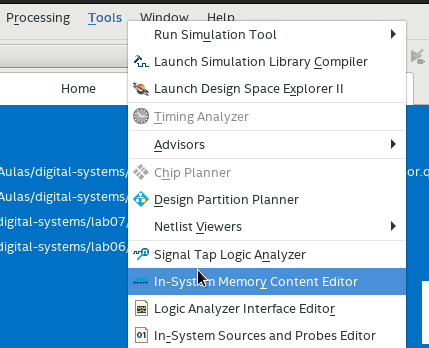
\includegraphics[width=.4\textwidth]{./images/memory_editor.png}
	\caption{Acesso ao editor de memória pelo menu do Quartus}
	\label{fig:editor}
\end{figure}

Para acessar o editor de memória foi necessário habilitar a funcionalidade durante a criação da entidade
da ram de uma porta pelo catálogo IP. Essa opção está marcada com um "x" vermelho na figura \ref{fig:enable_editor}.

\begin{figure}[ht]
	\centering
	\includegraphics[width=\textwidth]{./images/enable_editor.png}
	\caption{Opção para habilitar o editor de memória}
	\label{fig:enable_editor}
\end{figure}

\newpage
\section{Conclusão e comentários adicionais}
Foi utilizado nesse projeto a maioria dos conceitos estudados durante o semestre.
Conhecimento sobre memórias, lógica combinacional, registradores e máquinas de estado foram necessários para esse projeto.
O processador desenvolvido é um modelo simplificado, porém já serve como base para o estudo mais aprofundado 
que é ementa de disciplinas futuras sobre arquitetura de computadores.

Os códigos, descrições VHDL e programa de exemplo, estão disponíveis no diretório do projeto.



\newpage
\printbibliography

\end{document}
